\documentclass{article}
\usepackage[top=0pt,left=0pt,bottom=0pt,right=0pt,paperwidth=10cm,paperheight=5.4cm]{geometry}
\usepackage{tikz}
\usetikzlibrary{patterns.meta,decorations.pathmorphing}
\pagestyle{empty}
\begin{document}
\centering\vspace*{\fill}%
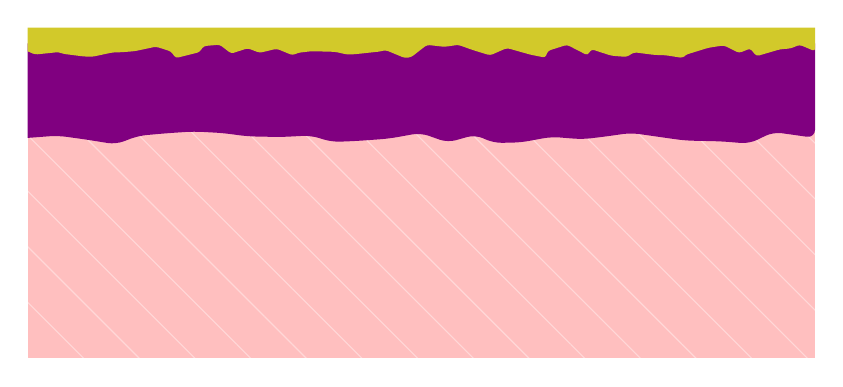
\begin{tikzpicture}
\path[use as bounding box] (-5,-1) rectangle (5,3.2);
\fill[pink,postaction={pattern={Lines[angle=-45,distance=5mm]},pattern color=white,opacity=0.4}] (-5,2) rectangle ++(10,-3);
\fill[violet] (-5,1.8) 
  decorate [decoration={random steps,segment length=10pt}, rounded corners=3pt] { -- ++(10,0) } 
  -- ++(0,1.2) -- ++(-10,0) -- cycle;
\fill[yellow!80!black] (-5,2.9) 
  decorate [decoration={random steps,segment length=5pt}, rounded corners=1pt] { -- ++(10,0) } 
  -- ++(0,0.3) -- ++(-10,0) -- cycle;
\end{tikzpicture}
\end{document}
